\documentclass[12pt, a4paper]{article}
\usepackage[utf8]{inputenc}
\usepackage{ctex}
\usepackage{geometry}
\usepackage{amsmath}
\usepackage{CJKutf8}
\usepackage{listingsutf8}
\usepackage{amssymb}
\usepackage{hyperref}
\usepackage{cite}
\usepackage{listings}
\usepackage{fancyhdr} % For headers and footers
\usepackage{lipsum} % For dummy text (remove this line)
\usepackage{float}
\usepackage{listings}
\usepackage{xcolor}
\usepackage{array} % 导入 array 宏包
\usepackage{verbatim} % 导入 verbatim 宏包
\usepackage{calc}
\usepackage{graphicx} % 支持图像处理
\usepackage{subcaption} % 支持子图环境

\lstset{
    basicstyle=\ttfamily,
    literate={├}{|---}{1} {─}{---}{1} {│}{|}{1} {└}{|___}{1},
    breaklines=true
}

\lstset{
    inputencoding=utf8,
    extendedchars=true,
    literate={一}{\CJKchar{"4E}{9C}}1 {二}{\CJKchar{"4E}{8C}}1 {三}{\CJKchar{"4E}{09}}1
    % Add more character mappings as needed
}

\definecolor{codegreen}{rgb}{0,0.6,0}
\definecolor{codegray}{rgb}{0.5,0.5,0.5}
\definecolor{codepurple}{rgb}{0.58,0,0.82}
\definecolor{backcolour}{rgb}{0.95,0.95,0.92}

\lstdefinelanguage{Makefile}{
    morekeywords = {all, clean, install, uninstall, verify, compile, run, png2bmp, python, make, verilator},
    sensitive = true,
    morecomment = [l]{\#},
    morestring = [b]",
}

\lstdefinestyle{mystyle}{
	commentstyle=\color{codegreen},
	keywordstyle=\color{magenta},
	numberstyle=\tiny\color{codegray},
	stringstyle=\color{codepurple},
	basicstyle=\ttfamily\footnotesize,
	breakatwhitespace=false,         
	breaklines=true,                 
	captionpos=b,                    
	keepspaces=true,                 
	numbers=left,                    
	numbersep=5pt,                  
	showspaces=false,                
	showstringspaces=false,
	showtabs=false,                  
	tabsize=2
}

\lstset{style=mystyle}

% 页面设置
\geometry{left=3cm,right=3cm,top=3cm,bottom=3cm}

% 标题和作者信息
\title{用Verilog语言实现把lena图像逆时针旋转90度}
\author{何天阳 $\quad$ 熊荣宇}
\date{\today}

\begin{document}

\maketitle

\section{引言}
本项目旨在通过Verilog语言实现对图像的路径描述,具体任务是将lena图像(或其他图像,
尺寸为256*256或512*512像素)进行90度逆时针旋转。

报告中包括:

1.部分原代码、仿真结果、工作报告与工作总结。

2.对非256*256*24bit格式的BMP图像进行格式转换,并确保输出图像尺寸为256*256像素。

3.详细记录设计中的输入输出信号、像素数据处理以及同步方式,确保输出图像的正确性。

\section{模块设计}

\begin{figure}[H]
    \centering
    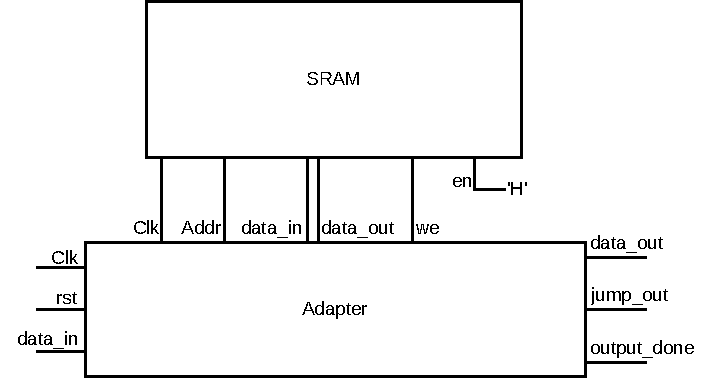
\includegraphics[width=0.8\textwidth]{images/struct.pdf}
    \caption{adapter模块设计}
    \label{fig:adapter}
\end{figure}

如图.~\ref{fig:adapter}所示,整体模块设计分为SRAM与Adapter两个部分。SRAM负责输入图像数据的存储,Adapter负责输入流程控制与数据存储的控制,控制整个流程。


\section{工作内容}

\subsection{环境搭建}

\noindent\textbf{构建运行流程}

由于需要读取与保存BMP图片格式,考虑到c++对于文件操作的便利性以及其生态的丰富,本次实验选择了Verilator编译器,该编译器可以将Verilog模块编译为C++以供测试代码调用仿真。

为了简化编译与运行的流程,这里使用了GNUMake,在Makefile中指定了项目构建的流程与步骤的依赖关系。

\begin{lstlisting}[language=Makefile]
TOP_MODULE=adapter
BUILD_DIR=obj_dir
# Scan All Source Code
VERILOG_SRC=$(wildcard ./src/*.v)
CPP_SRC=$(wildcard *.cpp *.hpp)
# Verilog Compile Parameters
VERILOG_FLAGS= --cc --exe -Wall --top-module $(TOP_MODULE)

all: run

# Verify Verilog Module
verify: $(VERILOG_SRC)
    verilator $(VERILOG_FLAGS) $(VERILOG_SRC) $(CPP_SRC)
# Compile Project
compile: verify
    make -j -C $(BUILD_DIR) -f V$(TOP_MODULE).mk V$(TOP_MODULE)

# Run Simulation
run: compile png2bmp
    ./$(BUILD_DIR)/V$(TOP_MODULE)

# Convert png to bmp with 24bit (RGB channels)
png2bmp: res/lenna.png
    python converter.py ./res/lenna.png


clean:
    rm -rf $(BUILD_DIR)
    rm ./output_lenna.bmp
    rm ./res/lenna.bmp
    rm ./output.bmp
    
\end{lstlisting}

\noindent\textbf{图片转换脚本}

由于网络下载的Lenna图片多为png,且格式可能不满足要求,使用python脚本与Pillow库完成图片格式的标准化转换。脚本如下:
\begin{lstlisting}[language=python]
import sys
from PIL import Image
import os

def convert_png_to_bmp(input_path, size=(256, 256)):
    output_path = os.path.splitext(input_path)[0] + ".bmp"
    with Image.open(input_path) as img:
        img = img.resize(size, Image.LANCZOS)
        img.save(output_path, format="BMP")

    print(f"Converted image saved to {output_path}")

if len(sys.argv) != 2:
    print("Usage: python convert.py <input_path>")
    sys.exit(1)

input_path = sys.argv[1]
convert_png_to_bmp(input_path)
\end{lstlisting}

\noindent\textbf{图片读入}

为了方便快速的读取BMP文件,使用第三方STBI库完成读取操作。使用git submodule来管理第三方库

\noindent\textbf{项目结构}

综上所述 项目结构大致如下文件树所示

\begin{lstlisting}
converter.py 
external  
Makefile  
obj_dir   
output_lenna.bmp
res       
src       
test.cpp  
\end{lstlisting}


\subsection{Verilog实现}

如图~\ref{fig:adapter} 所示的架构,SRAM负责输入图像数据的存储,而Adapter负责输入流程控制和数据存储控制。

对于RAM模块,首先定义输入的时钟周期信号Clk、使能信号en和写使能信号we,以及像素对应的地址addr和像素参数date\_in,输出的像素参数date\_out。

在时钟周期的上升沿,如果使能信号en为高电平,若输入输出信号we为高电平则给mem[addr]赋值data\_in,若输入输出信号en为低电平则将mem[addr]赋值给data\_out。

代码使用给出的参考代码,具体实现如下:
\begin{lstlisting}[language=verilog]
`define RAM_WIDTH 32 // Width of RAM
`define RAM_DEPTH 1024*1024 // Depth of RAM
`define ADDR_SZ 20 // Size of RAM address

module sram(
    clk,
    en, we,
    addr,
    data_in, data_out
);
    input clk, en, we;
    input [`ADDR_SZ-1:0] addr;
    input [`RAM_WIDTH-1:0] data_in;
    output reg [`RAM_WIDTH-1:0] data_out;

    reg [`RAM_WIDTH-1:0] mem [`RAM_DEPTH-1:0];

    always @(posedge clk) begin
        if (en) begin
            if (we) begin
                mem[addr] <= data_in;
            end
            else begin
                data_out <= mem[addr];
            end
        end
    end

endmodule : sram
\end{lstlisting}

adapter模块主要实现了图像的90度逆时针旋转,包括输入信号的存储,信号的处理和信号输出,
功能分解如下。

\subsubsection{输入输出端口}

\noindent\textbf{输入设计}
\begin{enumerate}
    \item 复位信号rst
    \item 输入输出模式切换mode
    \item 时钟信号clk
    \item 数据信号线data\_in
\end{enumerate}

\noindent\textbf{输出共设计}
\begin{enumerate}
    \item 数据输出信号data\_out
    \item 输出换行信号jump\_out
    \item 输出完成信号output\_done
\end{enumerate}

将Adapter设计为一个状态机, 设计两状态。1. State代表当前读入读出状态;2. 、
Coord(实际使用x,y两寄存器)代表当前的坐标状态,使用两个always块实现状态机。


\noindent\textbf{在第一个always块中,控制状态的切换和输出换行信号与输出完成信号的设置。}
\begin{lstlisting}[language=verilog]
always @(posedge clk or posedge rst) begin
    if (rst) begin
        x <= 0;
        y <= 0;
        jump_out <= 0;
        output_done <= 0; // Initialize output_done
    end else begin
        x <= next_x;
        y <= next_y;
        jump_out <= (next_x == 8'd255) ? 1'b1:1'b0;
        output_done <= (next_x == 8'd255 && next_y == 8'd255 && mode == 1'b1) ? 1'b1:0;
    end
end
\end{lstlisting}


\noindent\textbf{第二个always块根据当前输入引脚的状态, 设置next\_state。xy逐行输入,当到达行尾进行换行。此处完成了经典的两段式状态机的实现。}
\begin{lstlisting}[language=verilog]
always @(*) begin
    if (mode == 1'b0) begin
        if (x == 8'd255) begin
            next_x = 0;
            next_y = y+1;
        end else begin
            next_x = x+1;
            next_y = y;
        end
    end else begin
        if (x == 8'd255) begin
            next_x = 0;
            next_y = y+1;
        end else begin
            next_x = x+1;
            next_y = y;
        end
    end
end
\end{lstlisting}

\noindent\textbf{SRAM连接部分,将en保持置高,we与mode连接,共用时钟信号。}
\begin{lstlisting}[language=verilog]
sram ram(
    .clk(clk),
    .en(1'b1),
    .we(~mode),
    .addr(addr),
    .data_in(mem_in),
    .data_out(mem_out)
);
\end{lstlisting}

\noindent\textbf{其余线路与图像旋转部分直接使用assign连接}
\begin{lstlisting}
    assign addr = (mode == 1'b0) ? {4'b0, x, y}:{4'b0, 8'd255-y, x};
    assign mem_in = {8'b0, data_in};
    assign data_out = mem_out[23:0];
\end{lstlisting}

上述代码中,当mode处于读入模式时,正常读入坐标,当mode处于输出模式时,进行图片旋转的坐标映射:
\begin{equation*}
    (x',y') = (\text{size}-y, x)
\end{equation*}



\noindent\textbf{综上,全部代码如下:}
\begin{lstlisting}[language=verilog]
module adapter(
    input rst,
    input mode,
    input clk,
    input [23:0] data_in, // 8bit-rgb image

    output reg [23:0] data_out,
    output reg jump_out,
    output reg output_done // New output signal
);

    reg [7:0] x, next_x;
    reg [7:0] y, next_y;
    reg [19:0] addr;
    reg [31:0] mem_in;

    /* verilator lint_off UNUSEDSIGNAL */
    reg [31:0] mem_out;

    sram ram(
        .clk(clk),
        .en(1'b1),
        .we(~mode),
        .addr(addr),
        .data_in(mem_in),
        .data_out(mem_out)
    );

    always @(posedge clk) begin
        $display("x: %d, y: %d, addr: %h, data_in: %h, data_out: %h, jump_out: %h, output_done: %b", x, y, addr, mem_in, mem_out, jump_out, output_done);
        $display("mode %b, next_x: %d, next_y: %d", mode, next_x, next_y);
    end

    always @(posedge clk or posedge rst) begin
        if (rst) begin
            x <= 0;
            y <= 0;
            jump_out <= 0;
            output_done <= 0; // Initialize output_done
        end else begin
            x <= next_x;
            y <= next_y;
            jump_out <= (next_x == 8'd255) ? 1'b1:1'b0;
            output_done <= (next_x == 8'd255 && next_y == 8'd255 && mode == 1'b1) ? 1'b1:0;
        end
    end

    always @(*) begin
        if (mode == 1'b0) begin
            if (x == 8'd255) begin
                next_x = 0;
                next_y = y+1;
            end else begin
                next_x = x+1;
                next_y = y;
            end
        end else begin
            if (x == 8'd255) begin
                next_x = 0;
                next_y = y+1;
            end else begin
                next_x = x+1;
                next_y = y;
            end
        end
    end

    // Transform the address for 90-degree rotation
    assign addr = (mode == 1'b0) ? {4'b0, x, y}:{4'b0, 8'd255-y, x};
    assign mem_in = {8'b0, data_in};
    assign data_out = mem_out[23:0];
endmodule
    \end{lstlisting}

\subsection{TestBench 实现}

TestBench模块主要功能是验证Verilog模块的正确性。为了简便性,这里使用了Verilator编译器,该编译器可以将Verilog编译为C++以供仿真验证。

C++部分,使用了外部STBI库对图片进行读入和写入的操作。实例化Verilated对象,获取Top的Verilog模块,直接使用C++设置引脚数值,完成仿真流程的验证。

该部分较为简单,具体流程如下:

\begin{enumerate}
    \item 实例化Verilog模块。
    \item 读入BMP图片。
    \item 设置引脚为输入模式,循环时钟输入图片。
    \item 设置引脚为读取模式,循环时钟获取图片。
    \item 保存图片到文件。
\end{enumerate}


代码如下:
\begin{lstlisting}[language=c++]
#define STB_IMAGE_IMPLEMENTATION
#include "../external/stb/stb_image.h"
#define STB_IMAGE_WRITE_IMPLEMENTATION
#include "../external/stb/stb_image_write.h"

#include "Vadapter.h"
#include "verilated.h"

#include <iostream>
#include <fstream>
#include <vector>
#include <cstdint>

using namespace std;

bool readBMP(const char* filename, vector<uint8_t>& image, int& width, int& height, int& channels) {
    unsigned char* data = stbi_load(filename, &width, &height, &channels, 3);
    if (!data) {
        cerr << "Error: Could not open the file." << endl;
        return false;
    }

    image.assign(data, data + width * height * 3);
    stbi_image_free(data);
    return true;
}

bool writeBMP(const char* filename, const vector<uint8_t>& image, int width, int height) {
    if (stbi_write_bmp(filename, width, height, 3, image.data()) == 0) {
        cerr << "Error: Could not create the output file." << endl;
        return false;
    }
    return true;
}

int main(int argc, char **argv) {
    VerilatedContext *contextp = new VerilatedContext;
    contextp->commandArgs(argc, argv);
    Vadapter *top = new Vadapter{contextp};

    vector<uint8_t> image;
    int width, height, channels;

    if (!readBMP("./res/lenna.bmp", image, width, height, channels)) {
        return -1;
    }

    vector<uint8_t> output_data;
    output_data.resize(image.size());

    top->rst = 1;
    top->clk = 0;
    top->eval();
    top->rst = 0;
    top->eval();


    // Write image data into the Verilog module
    for (int y = 0; y < height; ++y) {
        for (int x = 0; x < width; ++x) {
            int index = (y * width + x) * 3;
            uint8_t r = image[index + 0];
            uint8_t g = image[index + 1];
            uint8_t b = image[index + 2];
            top->data_in = (r << 16) | (g << 8) | b;
            std::cout << std::hex << top->data_in << std::endl;
            top->eval();
            top->clk = 1;
            top->eval();
            top->clk = 0;
            top->eval();

        }
    }


    // Switch to read mode
    top->rst = 1;
    top->mode = 1;
    top->eval();
    top->rst = 0;
    top->mode = 1;
    top->eval();

    int index = 0;
    // Read image data from the Verilog module
    // Read image data from the Verilog module
    for (int y = 0; y < height; ++y) {
        for (int x = 0; x < width; ++x,index+=3) {
            top->eval();
            top->clk = 1;
            top->eval();
            output_data[index + 0] = (top->data_out >> 16) & 0xFF; // R
            output_data[index + 1] = (top->data_out >> 8) & 0xFF;  // G
            output_data[index + 2] = top->data_out & 0xFF;         // B
            top->clk = 0;
            top->eval();
        }
    }

    // Save output data to BMP file
    if (!writeBMP("output_lenna.bmp", output_data, width, height)) {
        return -1;
    }

    delete top;
    delete contextp;
    return 0;
}
\end{lstlisting}

\section{结果与分析}
经过运行,$lena$的原图和逆时针选转90度后$lena$的图像如下:

\begin{figure}[H]
    \centering
    \begin{minipage}[b]{0.45\textwidth}
        \centering
        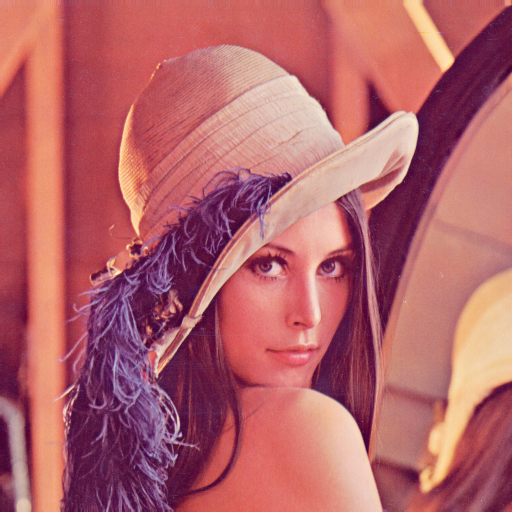
\includegraphics[width=1\textwidth]{images/lenna.png}
        \caption{lenna.bmp}
        \label{fig:lenna}
    \end{minipage}
    \hfill
    \begin{minipage}[b]{0.45\textwidth}
        \centering
        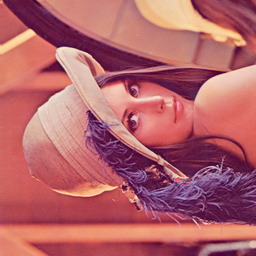
\includegraphics[width=1\textwidth]{images/output_lenna.png} 
        \caption{lenna.bmp}
        \label{fig:lenna_output}
    \end{minipage}
\end{figure}

\section{个人工作总结}
本次小组工作共有两名组员参与:何天阳、熊荣宇,以下为各自的个人工作总结。

\subsection{何天阳个人工作总结}

在本组项目中,我主要完成了$Verilog$模块部分编写,用于将$lena$图像逆时针旋转90度;以及分析了$testbench$的测试结果,撰写了项目报告。

在本项目中,我通过参与$Verilog$模块的编写和测试,我深入理解了图像处理算法在硬件层面的实现方法,学会了如何使用Verilog进行仿真与验证与其他编程语言的交互和引用方法。通过团队合作,提升了沟通协调能力,提高了在团队中分工合作,共同解决技术问题和项目挑战的能力。

\subsection{熊荣宇个人工作总结}

在本次项目中,我主要完成了$Verilog$模块的部分编写,主要是数据传输和逻辑控制的编写。
我还完成了$testbench$关键组件的编写,以及报告相应内容的撰写。

在本项目中,我通过深入参与$Verilog$模块的开发和测试,我提升了对硬件设计和验证流程的
理解。提升了有效协作和沟通,尤其是在技术讨论和解决问题时的团队合作能力。
我还收获了宝贵的实践经验,对未来的硬件开发项目有了更加自信的态度和准备。

\end{document}
